\documentclass[14pt]{beamer}
\usepackage[T2A]{fontenc}
\usepackage[utf8]{inputenc}
\usepackage[english,russian]{babel}
\usepackage{amssymb,amsfonts,amsmath,mathtext}
\usepackage{cite,enumerate,float,indentfirst}
\usepackage{makecell}
\usepackage{graphicx}
\graphicspath{{../images/}{images/}{../Thesis/images/}} 
\usepackage{tikz}
\usepackage{calc}
\def\checkmark{\tikz\fill[scale=0.7](0,.35) -- (.25,0) -- (1,.7) -- (.25,.15) -- cycle;}
\def\checkmarksmall{\tikz\fill[scale=0.5](0,.35) -- (.25,0) -- (1,.7) -- (.25,.15) -- cycle;}
\newcommand{\cond}{\;|\;}


%\usetheme[secheader]{Boadilla}
%\usecolortheme{seahorse}

\usetheme{Pittsburgh}
\usecolortheme{whale}



\beamertemplatenavigationsymbolsempty

\newcommand{\todo}{\alert}
%%% Основные сведения %%%
\newcommand{\thesisAuthorLastName}{Кочуров}
\newcommand{\thesisAuthorOtherNames}{Максим Вадимович}
\newcommand{\thesisAuthorInitials}{М.В.}
\newcommand{\thesisAuthor}             % Диссертация, ФИО автора
{%
    \texorpdfstring{% \texorpdfstring takes two arguments and uses the first for (La)TeX and the second for pdf
        \thesisAuthorLastName~\thesisAuthorOtherNames% так будет отображаться на титульном листе или в тексте, где будет использоваться переменная
    }{%
        \thesisAuthorLastName, \thesisAuthorOtherNames% эта запись для свойств pdf-файла. В таком виде, если pdf будет обработан программами для сбора библиографических сведений, будет правильно представлена фамилия.
    }
}
\newcommand{\thesisAuthorShort}        % Диссертация, ФИО автора инициалами
{\thesisAuthorInitials~\thesisAuthorLastName}
%\newcommand{\thesisUdk}                % Диссертация, УДК
%{\todo{xxx.xxx}}
\newcommand{\thesisTitle}              % Диссертация, название
{Эконометрическое моделирование динамики корреляций доходностей финансовых стратегий}
\newcommand{\thesisSpecialtyNumber}    % Диссертация, специальность, номер
{38.03.01}
\newcommand{\thesisSpecialtyTitle}     % Диссертация, специальность, название
{Экономика}
\newcommand{\thesisDegree}             % Диссертация, ученая степень
{Бакалавр Экономики}
\newcommand{\thesisDegreeShort}        % Диссертация, ученая степень, краткая запись
{Бакалавр Экономики}
\newcommand{\thesisCity}               % Диссертация, город написания диссертации
{Москва}
\newcommand{\thesisYear}               % Диссертация, год написания диссертации
{2018}
\newcommand{\thesisOrganization}       % Диссертация, организация
{Московский государственный университет имени М.В.Ломоносова}
\newcommand{\thesisOrganizationShort}  % Диссертация, краткое название организации для доклада
{МГУ им. М.В.Ломоносова}

\newcommand{\thesisInOrganization}     % Диссертация, организация в предложном падеже: Работа выполнена в ...
{Московском государственном университете имени М.В.Ломоносова}

\newcommand{\supervisorFio}            % Научный руководитель, ФИО
{Лукаш Евгений Николаевич}
\newcommand{\supervisorRegalia}        % Научный руководитель, регалии
{доцент кандидат экономических наук}
\newcommand{\supervisorFioShort}       % Научный руководитель, ФИО
{Е.Н. Лукаш}
\newcommand{\supervisorRegaliaShort}   % Научный руководитель, регалии
{доцент к.э.н.}


\newcommand{\opponentOneFio}           % Оппонент 1, ФИО
{\todo{Фамилия Имя Отчество}}
\newcommand{\opponentOneRegalia}       % Оппонент 1, регалии
{\todo{доктор физико-математических наук, профессор}}
\newcommand{\opponentOneJobPlace}      % Оппонент 1, место работы
{\todo{Не очень длинное название для места работы}}
\newcommand{\opponentOneJobPost}       % Оппонент 1, должность
{\todo{старший научный сотрудник}}

\newcommand{\opponentTwoFio}           % Оппонент 2, ФИО
{\todo{Фамилия Имя Отчество}}
\newcommand{\opponentTwoRegalia}       % Оппонент 2, регалии
{\todo{кандидат физико-математических наук}}
\newcommand{\opponentTwoJobPlace}      % Оппонент 2, место работы
{\todo{Основное место работы c длинным длинным длинным длинным названием}}
\newcommand{\opponentTwoJobPost}       % Оппонент 2, должность
{\todo{старший научный сотрудник}}

\newcommand{\leadingOrganizationTitle} % Ведущая организация, дополнительные строки
{\todo{Федеральное государственное бюджетное образовательное учреждение высшего профессионального образования с~длинным длинным длинным длинным названием}}

\newcommand{\defenseDate}              % Защита, дата
{23 мая 2018~г.}
\newcommand{\defenseCouncilNumber}     % Защита, номер диссертационного совета
{\todo{Д\,123.456.78}}
\newcommand{\defenseCouncilTitle}      % Защита, учреждение диссертационного совета
{\todo{Название учреждения}}
\newcommand{\defenseCouncilAddress}    % Защита, адрес учреждение диссертационного совета
{\todo{Адрес}}
\newcommand{\defenseCouncilPhone}      % Телефон для справок
{\todo{+7~(0000)~00-00-00}}

\newcommand{\defenseSecretaryFio}      % Секретарь диссертационного совета, ФИО
{\todo{Фамилия Имя Отчество}}
\newcommand{\defenseSecretaryRegalia}  % Секретарь диссертационного совета, регалии
{\todo{д-р~физ.-мат. наук}}            % Для сокращений есть ГОСТы, например: ГОСТ Р 7.0.12-2011 + http://base.garant.ru/179724/#block_30000

\newcommand{\synopsisLibrary}          % Автореферат, название библиотеки
{\todo{Название библиотеки}}
\newcommand{\synopsisDate}             % Автореферат, дата рассылки
{\todo{DD mmmmmmmm YYYY года}}

% To avoid conflict with beamer class use \providecommand
\providecommand{\keywords}%            % Ключевые слова для метаданных PDF диссертации и автореферата
{}
      % Основные сведения

\setbeamercolor{footline}{fg=blue}
\setbeamertemplate{footline}{
  \leavevmode%
  \hbox{%
  \begin{beamercolorbox}[wd=.333333\paperwidth,ht=2.25ex,dp=1ex,center]{}%
    % И. О. Фамилия, Организация кратко
    \thesisAuthorShort, \thesisOrganizationShort
  \end{beamercolorbox}%
  \begin{beamercolorbox}[wd=.333333\paperwidth,ht=2.25ex,dp=1ex,center]{}%
    % Город, 20XX
    \thesisCity, \thesisYear
  \end{beamercolorbox}%
  \begin{beamercolorbox}[wd=.333333\paperwidth,ht=2.25ex,dp=1ex,right]{}%
  Стр. \insertframenumber{} из \inserttotalframenumber \hspace*{2ex}
  \end{beamercolorbox}}%
  \vskip0pt%
}

\newcommand{\itemi}{\item[\checkmark]}

\title{\small{\thesisTitle}}
\author{\small{%
\emph{Выступающий:}~\thesisAuthorShort\\%
\emph{Руководитель:}~\supervisorRegaliaShort~\supervisorFioShort}\\%
\vspace{30pt}%
\thesisOrganization%
\vspace{20pt}%
}
\date{\small{\thesisCity, \thesisYear}}

\begin{document}
\maketitle
\begin{frame}{Актуальность}
\textbf{Актуальность:}
\begin{itemize}
	\item Торговые алгоритмы -- альтернатива активам
	\item Алгоритмы могут реагировать на шоки*
	\item Портфель из торговых стратегий -- возможность лучшей диверсификации
\end{itemize}
* Обыграть рынок -- не цель, важно разнообразие
\vspace{\baselineskip}

\textbf{Предмет исследования} -- приложение портфельной теории для составления портфеля торговых стратегий.
\end{frame}
\begin{frame}{Цели и Задачи}

\textbf{Проблемы:}
\begin{itemize}
	\item Алгоритмы $\ne$ Активы
	\item Алгоритмов много (>700000), нужен отбор
	\item Их составляют люди $\rightarrow$ <<переобучение>>
	\item[$\blacktriangleright$] Много априорных знаний не про структуру
\end{itemize}
\vspace{\baselineskip}

\textbf{Цель:} учесть априорные знания о доходностях алгоритмов при формировании портфеля торговых стратегий
\end{frame}
\begin{frame}{Цели и Задачи}
\textbf{Задачи:}
\begin{itemize}
	\item Предложить модель динамики доходности ТС
	\item Предложить способ составления портфеля
	\item Провесит сравнительный анализ для разработанного метода
\end{itemize}
\visible<2>{
\underline{\textbf{Структура работы}}
\begin{itemize}
	\item[>] Описание проблемы
	\item[>] Обзор и адаптация существующих методов
	\item[>] Эмпирическая часть, сравнительный анализ
\end{itemize}
}
\end{frame}
\begin{frame}{Особенности Алгоритмов}
\textbf{Алгоритмы $\ne$ Активы}
\begin{itemize}
	\item Другая структура рисков
	\item Комиссия за транзакции
\end{itemize}
\textbf{Происхождение алгоритмов}
\begin{itemize}
	\item Создаются авторами на спец. платформе
	\item Авторы видят результаты <<бэктеста>>
	\item Авторы конкурируют между собой
	\item[$\blacktriangleright$] Точка перелома, <<проблема оракула>>
\end{itemize}
\end{frame}
\begin{frame}{Байесовкий vs Частотный подход}
\resizebox{\linewidth}{!}{
\begin{tabular}{l|c|c}
	& Байесовский  & Частотный \\ \hline
	Вероятность & мера знания & частота события \\ \hline
	\makecell{Параметры \\ модели}& случайные величины & неизвестные константы \\ \hline
	Данные & \multicolumn{2}{c}{из неизвестного распределения}  \\ \hline
	\makecell{Учет априорной \\ информации} & \qquad да \visible<2>{ \textcolor{green}{\checkmark}}& нет \\ \hline
	Размер выборки & $\forall$ & $\gg0$
\end{tabular}
}
\end{frame}
\begin{frame}{Учёт предпосылок}
\begin{itemize}
	\item Точка перелома
	\begin{itemize}
		\item[>] Структурный сдвиг -- часть модели 
	\end{itemize}
	\item<2-> Доходности имеют непостоянную волатильность (Dumas et al., 1998)
	\begin{itemize}
		\item[>] Модели волатильности: GARCH, \textcolor<3->{green}{GPVol}
	\end{itemize}
	\item<4-> Динамика корреляций (Vaga, 1990)
	\begin{itemize}
		\item[>] Модели динамической корреляции: DCC, \textcolor<5->{green}{DECO}
		\item<5->[>] Используем модификацию DECO
		\item<6-|alert@6>[>]Верно ли для доходностей стратегий?
	\end{itemize}
\end{itemize}
\end{frame}
\begin{frame}{Спецификация модели}
\textbf{Гауссовские процессы}

\begin{minipage}{.5\linewidth}
\begin{itemize}
	\item[+] Гибкость модели
	\item[+] Интерпретируемые параметры
	\item[+] Позволяют учесть априорные знания
\end{itemize}
\end{minipage}
\begin{minipage}{.48\linewidth}
	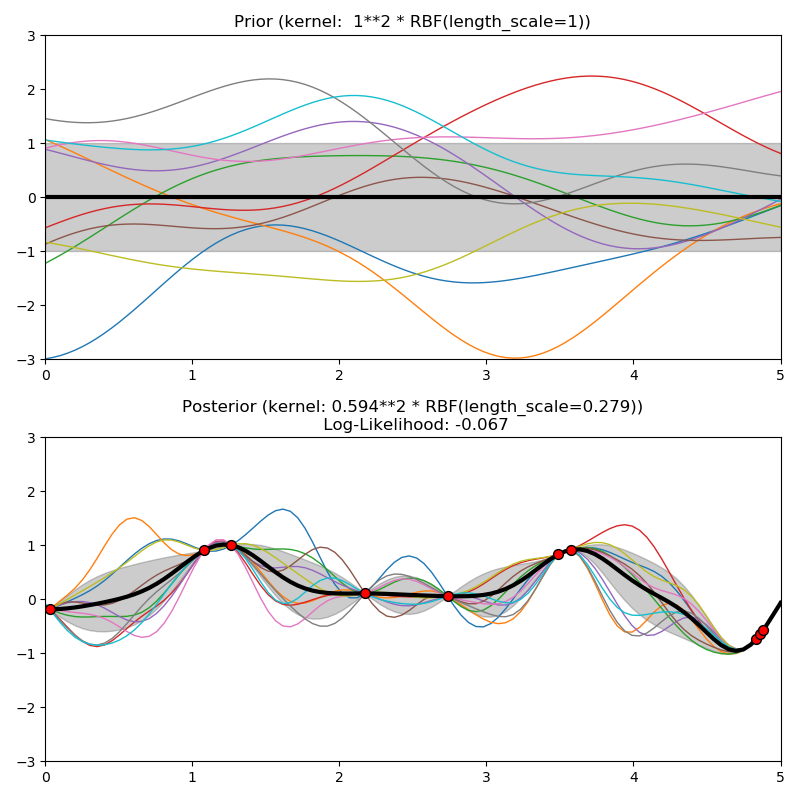
\includegraphics[width=\linewidth]{sampleGP}
\end{minipage}
\end{frame}
\begin{frame}{Спецификация модели}
\textbf{Ключевые идеи:}
\begin{itemize}
	\item Доходности $r_t$ $\sim$ Гауссовский Процесс + шум
	\begin{itemize}
		\item[\checkmarksmall] среднее ГП -- средняя доходность
		
		(о ней много знаем)
	\end{itemize}
	\item<2-> Волатильность $\sigma_t$ $\sim$ Гауссовский Процесс
	\begin{enumerate}
		\item[\checkmarksmall] Идеи GPVol
	\end{enumerate}
	\item<3-> Корреляции?
	\begin{enumerate}
		\item Динамические $\rightarrow$ модификация DECO с ГП
		\item Статические $\rightarrow$ $r_t \sim \mathcal{N}(\mu_t, LL^\top\odot\sigma_t\sigma_t^\top)$
		\item Без корреляций $\rightarrow$ $r_t \sim \mathcal{N}(\mu_t, diag(\sigma_t))$
	\end{enumerate}
	\item<4-> Структурный сдвиг
	\begin{itemize}
		\item[\checkmarksmall] только для средних доходностей
	\end{itemize}
\end{itemize}
\end{frame}
\begin{frame}{Оптимизация портфеля}
\textbf{Метод Монте Карло}

\begin{minipage}{0.49\linewidth}
	\begin{itemize}
		\item Оцениваем модель
		\item Делаем симуляции доходностей
		\item Оптимизируем матожидание функции полезности инвестора
	\end{itemize}
\end{minipage}
\begin{minipage}{0.49\linewidth}
	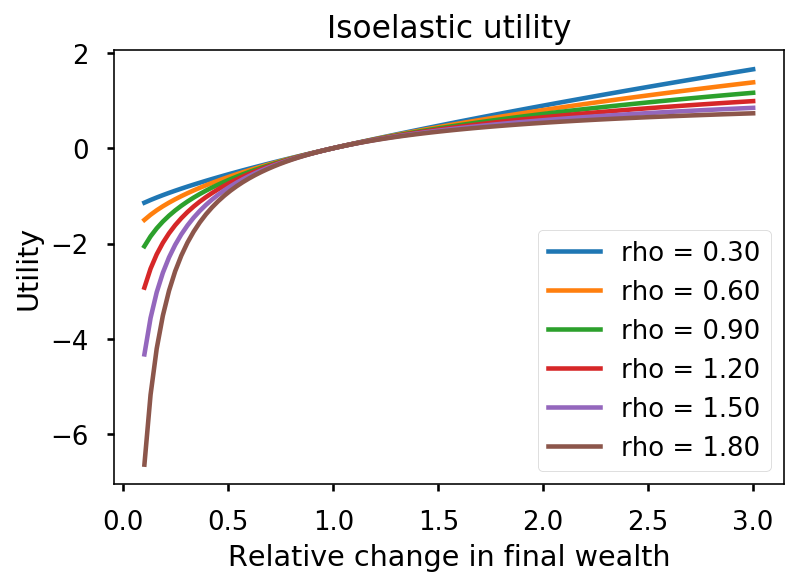
\includegraphics[width=\linewidth]{isoelastic}
	
	График: Полезность инвестора
\end{minipage}
\end{frame}
\begin{frame}{Оценка байесовской модели}
\textbf{Hamiltonian Monte Carlo}
\begin{tabular}{lr}
\includegraphics[height=2.5em]{pymc3}
&\makecell{\vspace{1.5em}
$\small p(\Theta\cond\mathcal{D}) =
\frac
{p(\mathcal{D}\cond\Theta)p(\Theta)}
{\color{red}{p(\mathcal{D})}}$}
\end{tabular}

\begin{minipage}{.5\linewidth}
	\begin{itemize}
		\item[+] Сэмплирование из сложных распределений
		\item[+] Хорошие условия сходимости
		\item[\checkmarksmall] Требуется непрерывность параметров
	\end{itemize}
\end{minipage}
\begin{minipage}{.48\linewidth}
	\includegraphics[width=\linewidth]{sampleHMC}
\end{minipage}
\end{frame}

\begin{frame}{Данные}
Данные были предоставлены компанией \textbf{Quantopian}\footnote{\vspace{.5em}В рамках стажировки}
\begin{itemize}
	\item Всего 700000+ алгоритмов за период 4 года
	\item Существует внутренняя система отбора стабильных алгоритмов
	\item Таких получается около 0.05\%
	\item Для исследования предоставлены 150 из них
\end{itemize}
\end{frame}

\begin{frame}{Проверка гипотез}
\textbf{Стохастическая волатильность}
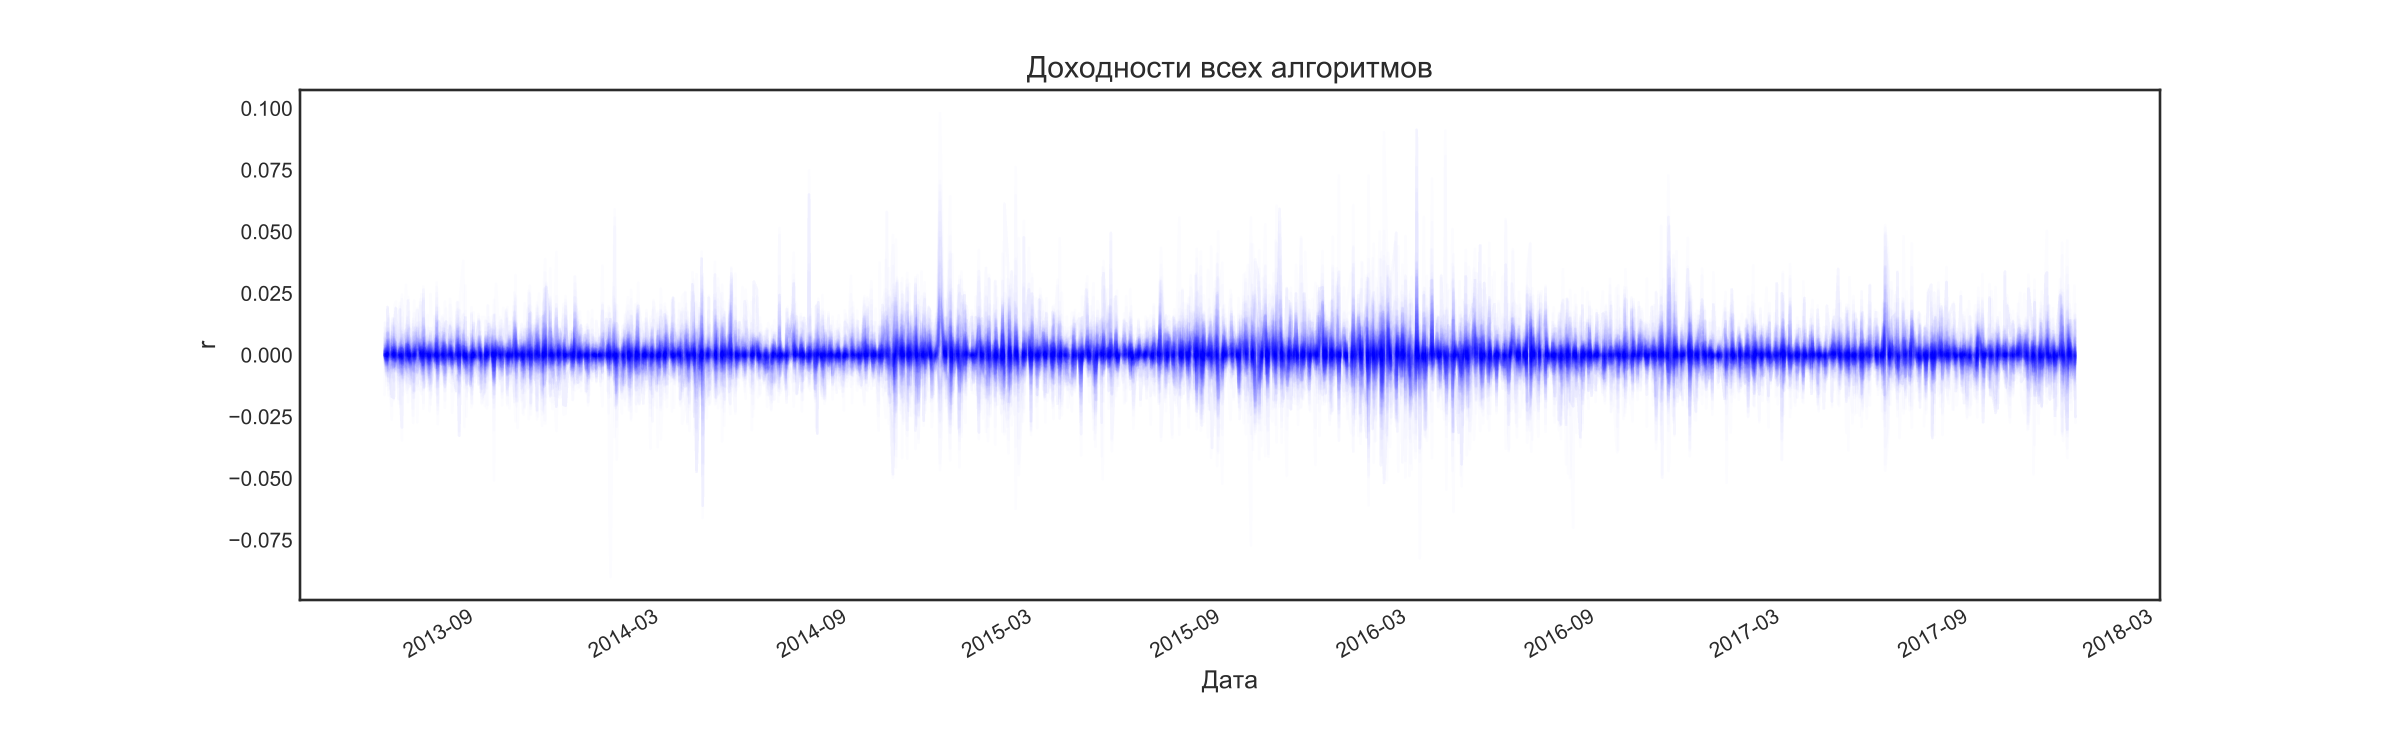
\includegraphics[width=\linewidth]{returns-all}

График: Распределение доходностей \textit{Всех} алгоритмов во времени
\begin{itemize}
	\item Наблюдается эффект стохастической волатильности
\end{itemize}
\end{frame}

\begin{frame}{Проверка гипотез}
\textbf{Динамика корреляций}
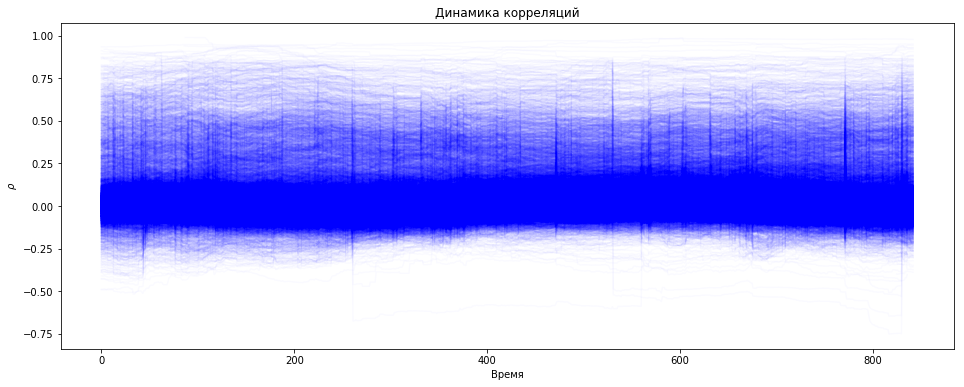
\includegraphics[width=\linewidth]{correlations}

График: Траектории скользящих корреляций доходностей алгоритмов
\begin{itemize}
	\item Корреляции довольно стабильны во времени
\end{itemize}
\end{frame}
\begin{frame}{Проверка гипотез}
\begin{itemize}
	\item Наблюдается эффект стохастической волатильности
	\item Корреляции довольно стабильны во времени
\end{itemize}
Подходят только спецификации со статическими корреляциями.

\end{frame}
\begin{frame}{Сравнительный анализ (бутстрэп)}
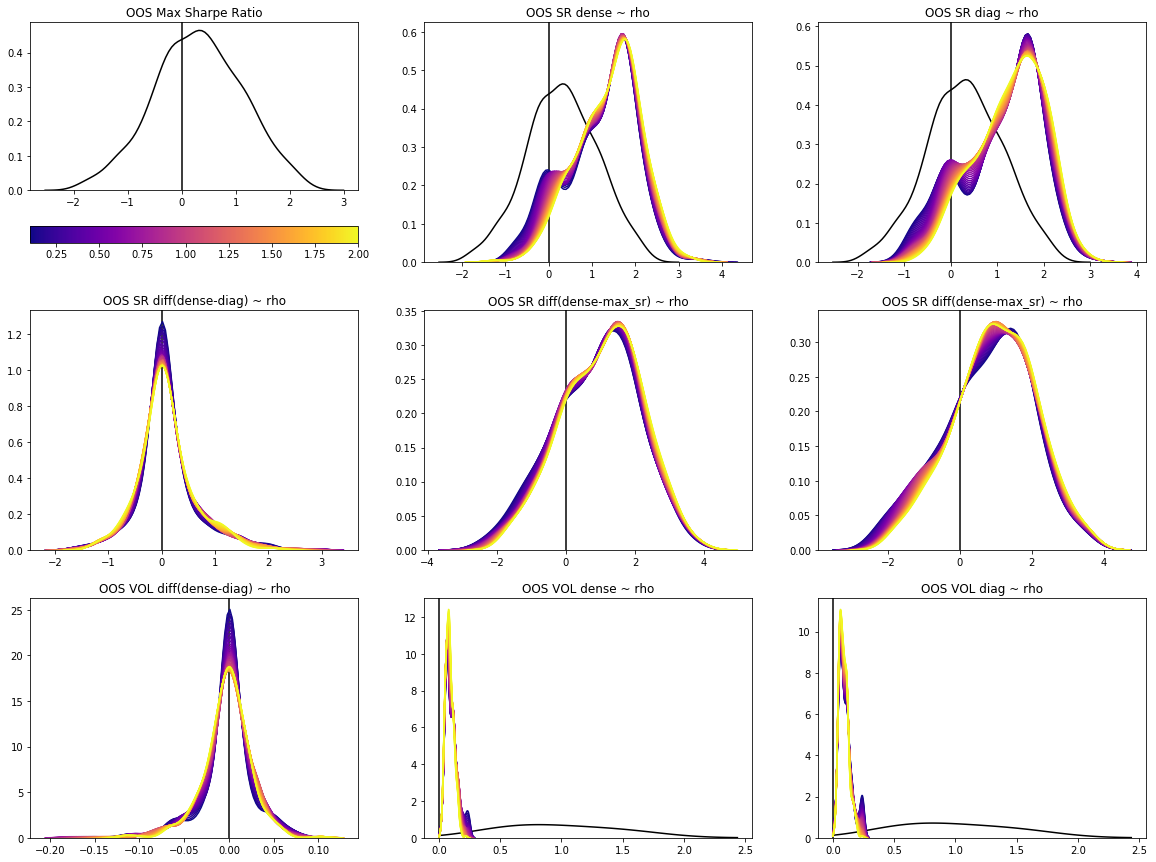
\includegraphics[width=.7\linewidth]{performance}
	
График: Сравнение коэффициента Шарпа полученного с использованием разных моделей для составления оптимального портфеля
\end{frame}
\begin{frame}{Заключение}
\begin{itemize}
	\item Предложен устойчивый подход к составлению портфеля торговых стратегий
	\item Предложена модификация базовых методов
	\item Реализован продукт успешно решающий прикладную задачу
\end{itemize}
\end{frame}
\end{document}
